\documentclass[]{article}
\usepackage{amsmath}
\usepackage{amsfonts}
\usepackage{amssymb}
\usepackage{hyperref}
\usepackage{gensymb}
\usepackage{graphicx}
\usepackage{svg}
\usepackage{bbding}
\usepackage{mathtools}
\usepackage{centernot} % not parallel, etc.
\usepackage{lmodern}
\usepackage{morewrites}
\usepackage{xcolor,sectsty} % colorful sections
\usepackage[left=10mm, top=10mm, right=10mm, bottom=20mm, nohead]{geometry}
%\usepackage{bigints}
\usepackage{dsfont} %mathbb 1
\usepackage{esint} % beatiful integrals
\usepackage{physics} % bra and ket


\DeclareFontFamily{OMX}{lmex}{}
\DeclareFontShape{OMX}{lmex}{m}{n}{<-> lmex10}{}


%colors of sections
\definecolor{secfont}{RGB}{46,116,181}
\definecolor{subfont}{RGB}{146,23,57}
\definecolor{parfont}{RGB}{19,127,43}
\definecolor{subparfont}{RGB}{7,11,100}

\subsectionfont{\color{subfont}}
\sectionfont{\color{secfont}}
\paragraphfont{\color{parfont}}
\subparagraphfont{\color{subparfont}}

%\usepackage{babel}[english]
%opening
\title{115203 - Quantum Physics 1}
\author{Amos Yarom}

\parindent=0em
\begin{document}


\maketitle

\begin{abstract}

\end{abstract}

%\tableofcontents
\section{Introduction}
\subsection{Stern–Gerlach experiment }
Suppose particles can be either black or white and we have some tool which can measure a color of particles. Additional, suppose, particles have additional property ''hardness` `- and we can measure whether particles are hard or soft.

The properties are consistent - i.e.\ it doesn't matter how many times you measure it one after other, you get the same result. Also, hardness and color are independent - if you measure hardness, you get either white or black with same probability.

The experiment itself is measuring color, then hardness, and then color again. Even though we input only white particles into hardness measuring tool, the output of second color measurement is either white or black with equal probability.

\paragraph{Principles of quantum mechanics}
\begin{enumerate}
	\item Particle is described with normalized vector in complex space of physical states.
	
	In our example, the space is 2D - black/white and hard/soft.
	\item Given system in (normalized) state $\vec{v}_1$, probability that it will be in state $\vec{v}_2$ is
	$$P = \left|\vec{v}_2 \cdot \vec{v}_1 \right|^2$$
	
	So, in our example, suppose $\hat{w}$ and $\hat{b}$ are orthogonal basis of our space. Since we know that 
	$$\begin{cases}
	\left|\vec{w} \cdot\vec{s}\right|^2 = \frac{1}{2}\\
	\left|\vec{b} \cdot\vec{s}\right|^2 = \frac{1}{2}\\
	\end{cases}$$
	We know that angle with both axis of $\vec{s}$ is $\frac{\pi}{4}$. We can choose any of 4 possibilities. Lets choose $\hat{s} = \frac{\hat{w} - \hat{b}}{\sqrt{2}}$ and since $\hat{h}$ is orthogonal, $\hat{h} = \frac{\hat{w} + \hat{b}}{\sqrt{2}}$.
\item Each measurement can be characterized with Hermitian operator, whose eigenvalues are outcomes of measurements and corresponding eigenvectors are states after the measuremnts.
\end{enumerate}

	
Now we can predict the results of opposite experiment - if we measure hardness of white particle, it will be hard with probability $\frac{1}{2}$. Now the probability that resulting hard particle will be measured to be white, is also $\frac{1}{2}$.

In quantum mechanics we use bra ket notation: vector is denoted $\ket{b}$ (conjugate transposed vector is denoted as $\bra{w}$):
$$\ket{h} = \frac{1}{\sqrt{2}} \ket{b} +  \frac{1}{\sqrt{2}} \ket{w}$$
\paragraph{Example}
Suppose we have a particle 
$$\ket{\Psi} = \frac{1}{\sqrt{3}} \ket{w} + \sqrt{\frac{2}{3}} \ket{b} $$
Then probability that it will be measured as white
$$P(w) = \left|\braket{w}{\Psi}\right|^2 = \left|\frac{1}{\sqrt{3}}\braket{w}{w} + \sqrt{\frac{2}{3}}\braket{w}{b}\right|^2 = \frac{1}{3} $$
If measure hardness:
$$P(h) = \left|\braket{h}{\Psi}\right|^2 = \left|\left(\frac{1}{\sqrt{2}} \ket{b} +  \frac{1}{\sqrt{2}} \ket{w}\right)\left(\frac{1}{\sqrt{3}} \ket{w} + \sqrt{\frac{2}{3}} \ket{b} \right)\right|^2 = \left| \frac{1}{\sqrt{3}} + \frac{1}{\sqrt{6}}\right| \approx 0.3$$
\section{Linear algebra}
\paragraph{Linear operator}
In quantum mechanics we write operators as multiplication of vectors. For example for
$$R = \begin{pmatrix}0&-1\\1&0\end{pmatrix}$$
we write
$$R = - \op{w}{b} + \op{b}{w}$$
And then
$$R\ket{\Psi} = - \ket{w}\braket{b}{\Psi} + \ket{b}\braket{w}{\Psi} = - \braket{b}{\Psi}\ket{w} + \braket{w}{\Psi} \ket{b}$$
For example
$$R\ket{s}= \ket{b}\braket{w}{s}-\ket{w}\braket{b}{s}=\ket{b}\frac{1}{\sqrt{2}}+ \ket{w}\frac{1}{\sqrt{2}} = \ket{h}$$

\paragraph{Examples}
\begin{itemize}
	\item $$W = \op{w}{b} + \op{w}{w}$$
	\item $$T = \op{h}{b} + \op{s}{w}$$
	\item $$Q = 2\op{w}{w} + 3\op{b}{b}$$
	This is not unitary operator, since in doesn't conserves norm.
\end{itemize}

\paragraph{Basis change}
To change from basis to basis we just substitute the values of old basis in a new one:
$$T = \ket{h} \left(\frac{1}{\sqrt{2}}\bra{h} - \frac{1}{\sqrt{2}}\bra{s}\right) + \ket{s} \left(\frac{1}{\sqrt{2}}\bra{h} + \frac{1}{\sqrt{2}}\bra{s}\right) =  \frac{1}{\sqrt{2}}\op{h}{h} - \frac{1}{\sqrt{2}}\op{h}{s} + \frac{1}{\sqrt{2}}\op{s}{h} + \frac{1}{\sqrt{2}}\op{s}{s}$$

\paragraph{Hermitian operators}
We want to build an operator $C$ such that for state $\ket{\psi}$ it will return us the average of $\psi$:
$$\braket{\psi|C}{\psi} = \langle \psi \rangle$$
If we give a value of $-1$ to white and value of $1$ to black:
$$\mel{\psi}{C}{\psi} = -1 \cdot P(\psi = w) + 1 \cdot P(\psi = b) = - \abs{\braket{w}{\psi}}^2 + \abs{\braket{b}{\psi}}^2 = -\braket{\psi}{w}\braket{w}{\psi}+\braket{\psi}{b}\braket{b}{\psi}$$
Thus
$$C = -\op{w}{w}+\op{b}{b}$$

For example, for $\psi = \frac{1}{\sqrt{3}}\ket{w} + \sqrt{\frac{2}{3}}\ket{b}$:
$$\mel{\psi}{C}{\psi} = \bra{\psi} \left( -\op{w}{w}+\op{b}{b} \right)\left( \frac{1}{\sqrt{3}}\ket{w} + \sqrt{\frac{2}{3}}\ket{b} \right) = \bra{\psi} \left(-\frac{1}{\sqrt{3}}\ket{w} + \sqrt{\frac{2}{3}}\ket{b}\right) = \frac{1}{3}$$


\paragraph{Additional example}
Suppose we have two properties - color and temperature. Possible values are red, green, blue for color and hot, lukewarm, cold for temperature.

If we measure temperature of red or green particle we get lukewarm of hot with equal probability. If we measure temperature of blue particle we get cold surely.

How can we write $\ket{b}$, $\ket{g}$, $\ket{r}$ in basis of $\ket{c}$, $\ket{l}$, $\ket{h}$?

From first experiment
$$\ket{r} =  \frac{1}{\sqrt{2}} \ket{l} + \frac{1}{\sqrt{2}} \ket{h} $$
$$\ket{g} =   \frac{1}{\sqrt{2}} \ket{l} - \frac{1}{\sqrt{2}} \ket{h} $$

Note that we need minus since else we'd get $\braket{g}{r} = 1$.
From last experiment
$$\ket{b}= \ket{c}$$

Lets denote $h=1$, $l=0$, $c=-1$ and build temperature operator. It's characterized by
$$\begin{cases}
T\ket{h} = \ket{h}\\
T\ket{l} = 0\\
T\ket{c} = -\ket{c}
\end{cases}$$
And thus an operator is
$$T = \op{h}{h} - \op{c}{c}$$

Now let's calculate temperature of state $\ket{g}$:
$$\mel{g}{T}{g} = \left(\frac{1}{\sqrt{2}} \ket{l} - \frac{1}{\sqrt{2}} \ket{h}\right)T \left(\frac{1}{\sqrt{2}} \ket{l} - \frac{1}{\sqrt{2}} \ket{h} \right) = \frac{1}{2}  \left(\ket{l} -\ket{h}\right)T \left( \ket{l} -\ket{h} \right) =-\frac{1}{2}  \left(\ket{l} -\ket{h}\right)\ket{h} = \frac{1}{2}  $$

We can also calculate variance:
$$\sigma^2 = \mel{g}{T^2}{g} - \big(\mel{g}{T}{g}\big)^2$$

\paragraph{Example}
We have a particle can be at one of five points. So possible states are $\ket{1}$,$\ket{2}$,$\ket{3}$,$\ket{4}$,$\ket{5}$.

If we want to describe a particle on finite 1D interval, we'll divide it into $N$ equal intervals of length $a$. We are interested in $a \to 0$, thus number of dimensions goes to infinity.

\paragraph{double slit experiment}
\input{lect3.tex}
\section{Tons of linear algebra}
...
\subsection{Fourier transform operator}
Define space with basis $\ket{x}$ such that $\braket{x}{f} = f(x)$ and $\braket{x}{x'} = \delta(x-x')$
Define identity operator
$$I = \int \dyad{x}{x} \dd{x}$$
Define also operator $K$ such that
$$\mel{x}{K}{f} = - i\pdv{f}{x}$$
$K$ is Hermitian if $\eval{f \vdot g}_a^b = 0$ for any $f$,$g$.

It's eigenvalues $k$ are such that
$$\braket{x}{k} = \frac{1}{\sqrt{2\pi}} e^{ikx}$$
Also for $f$
$$\ket{f} = \int f(x) \ket{x} \dd{x} = \int \hat{f} (k) \ket{k} \dd{k} $$
when
$$\braket{k}{f} = \hat{f}(k)$$

Define operator $X$ such that $X\ket{x} = x\ket{x}$. Obviously, $X$ is Hermitian.
$$\mel{x}{X}{f} = \qty(\mel{f}{X^\dagger}{x})^* =  \qty(\mel{f}{X}{x})^* = \qty(x\braket{f}{x})^* = x^* \braket{x}{f} = xf(x) $$

Lets calculate $\comm{X}{K}$:
$$\mel{x}{XK}{f} = \mel{x}{XIK}{f} = \int \mel{x}{X}{x'} \mel{x'}{K}{f} \dd{x'} = \int x'\delta(x-x') \qty(-i\pdv{f}{x'}) \dd{x'} = -ix \pdv{f}{x}$$
Now
$$\mel{x}{KX}{f} = \int \mel{x}{K}{x'} \mel{x'}{X}{f} \dd{x'} = \int -i \delta(x-x') \pdv{x'} \qty(x'f(x)) \dd{x'} = -i \pdv{x}\qty(xf(x)) = -if(x) -ix\pdv{f}{x}  $$
Thus
$$\mel{x}{\comm{X}{K}}{f} = -ix\pdv{f}{x} - \qty(-if(x) - ix\pdv{f}{x}) = if(x) = i\mel{x}{I}{f}$$
i.e.
$$\comm{X}{K} = iI$$

We suppose that our space is complete (i.e. each Cauchy sequence converges). Complete inner product space is called Hilbert space.

\section{Quantum mechanics principles}
\begin{enumerate}
	\item Physical state is described by vector $\ket{\psi}$ in Hilbert space
	\item Given state $\ket{\psi}$, probability to measure it in state $\varphi$ is
	$$P = \frac{\abs{\braket{\varphi}{\psi}}^2}{\braket{\varphi}{\varphi} \braket{\psi}{\psi}}$$
	\item Measurable quantities are described by Hermitian operator $\Omega$:
	\begin{enumerate}
		\item Result of measurement is one of eigenvalues of $\Omega$
		\item A state corresponding to measurement of value $\omega$ is $\ket{\omega}$.
		\item After measurements, the state will be corresponding eigenvector
	\end{enumerate} 
	\item Given state $\psi$ at $t=0$, a state at time $t$ is given by following PDE:
	$$i\hbar \pdv{t} \ket{\psi}  = H\ket{\psi}$$ 
	which is called Schr\"{o}dinger equation
\end{enumerate}

\paragraph{Position and momentum operators}
Position operator is $X$ and momentum operator $P = \hbar K$.
\paragraph{Consequences of principles}
\begin{enumerate}
	\item Particle on line is described with vector in infinite-dimensional space.
	\item If $\ket{\psi}$ and $\ket{\varphi}$ are physical states, $\ket{\varphi} + \ket{\psi}$ is physical state too.
	\item It's impossible to predict results of measurements, only probability of results.
	\item Norm of the vector is not important, since we always can normalize them.
	\item Results of measurements of $\Omega$ are only $\omega_i$.
	\item If $\ket{\psi} = \ket{\omega}$, such that $\Omega \ket{\omega} = \omega\ket{\omega}$ then measurement of $\Omega$ will always give $\omega$.
	\item Classical physical quantity which depends on $x$ and $p$, its quantum analogue is same function of operators $X$ and $P$: 
	$$\Omega(x,p) \Rightarrow \Omega(X,P)$$
	The order is important, since $\comm{X}{P} \neq 0$. Some operators are defined only in quantum case, e.g. $\Omega = \comm{X}{P}$. Thus the right way to proceed is to define quantum quantities and then to check what happens in classical limit.
	\item If there is degeneracy, i.e., some eigenvalue of the operator has multiple eigenvectors, the probability is a sum of probabilities:
	$$P = \abs{\braket{\omega,1}{\psi}}^2 + \abs{\braket{\omega,2}{\psi}}^2$$
\end{enumerate}
\paragraph{Expectation and variance of measurement}
Expectation of measurement can be calculated as
$$\mel{\psi}{\Omega}{\varphi} = \sum_i \omega_i P_\psi(\omega)$$
and variance
$$\Delta \Omega^2 = \mel{\psi}{\qty(\Omega - \mel{\psi}{\Omega}{\psi})^2}{\psi}$$
\subsection{Schr\"{o}dinger equation}
\paragraph{Examples of Hamiltonian}
For free particle
$$H = \frac{P^2}{2m}$$
For harmonic oscillator
$$H = \frac{P^2}{2m} + \frac{1}{2}\omega^2 X^2$$

Suppose Hamiltonian is independent on time. We want to diagonalize Hamiltomnian.
\subsection{Fourier transform operator}
Define space with basis $\ket{x}$ such that $\braket{x}{f} = f(x)$ and $\braket{x}{x'} = \delta(x-x')$
Define identity operator
$$I = \int \dyad{x}{x} \dd{x}$$
Define also operator $K$ such that
$$\mel{x}{K}{f} = - i\pdv{f}{x}$$
$K$ is Hermitian if $\eval{f \vdot g}_a^b = 0$ for any $f$,$g$.

It's eigenvalues $k$ are such that
$$\braket{x}{k} = \frac{1}{\sqrt{2\pi}} e^{ikx}$$
Also for $f$
$$\ket{f} = \int f(x) \ket{x} \dd{x} = \int \hat{f} (k) \ket{k} \dd{k} $$
when
$$\braket{k}{f} = \hat{f}(k)$$

Define operator $X$ such that $X\ket{x} = x\ket{x}$. Obviously, $X$ is Hermitian.
$$\mel{x}{X}{f} = \qty(\mel{f}{X^\dagger}{x})^* =  \qty(\mel{f}{X}{x})^* = \qty(x\braket{f}{x})^* = x^* \braket{x}{f} = xf(x) $$

Lets calculate $\comm{X}{K}$:
$$\mel{x}{XK}{f} = \mel{x}{XIK}{f} = \int \mel{x}{X}{x'} \mel{x'}{K}{f} \dd{x'} = \int x'\delta(x-x') \qty(-i\pdv{f}{x'}) \dd{x'} = -ix \pdv{f}{x}$$
Now
$$\mel{x}{KX}{f} = \int \mel{x}{K}{x'} \mel{x'}{X}{f} \dd{x'} = \int -i \delta(x-x') \pdv{x'} \qty(x'f(x)) \dd{x'} = -i \pdv{x}\qty(xf(x)) = -if(x) -ix\pdv{f}{x}  $$
Thus
$$\mel{x}{\comm{X}{K}}{f} = -ix\pdv{f}{x} - \qty(-if(x) - ix\pdv{f}{x}) = if(x) = i\mel{x}{I}{f}$$
i.e.
$$\comm{X}{K} = iI$$

We suppose that our space is complete (i.e. each Cauchy sequence converges). Complete inner product space is called Hilbert space.

\section{Quantum mechanics principles}
\begin{enumerate}
	\item Physical state is described by vector $\ket{\psi}$ in Hilbert space
	\item Given state $\ket{\psi}$, probability to measure it in state $\varphi$ is
	$$P = \frac{\abs{\braket{\varphi}{\psi}}^2}{\braket{\varphi}{\varphi} \braket{\psi}{\psi}}$$
	\item Measurable quantities are described by Hermitian operator $\Omega$:
	\begin{enumerate}
		\item Result of measurement is one of eigenvalues of $\Omega$
		\item A state corresponding to measurement of value $\omega$ is $\ket{\omega}$.
		\item After measurements, the state will be corresponding eigenvector
	\end{enumerate} 
	\item Given state $\psi$ at $t=0$, a state at time $t$ is given by following PDE:
	$$i\hbar \pdv{t} \ket{\psi}  = H\ket{\psi}$$ 
	which is called Schr\"{o}dinger equation
\end{enumerate}

\paragraph{Position and momentum operators}
Position operator is $X$ and momentum operator $P = \hbar K$.
\paragraph{Consequences of principles}
\begin{enumerate}
	\item Particle on line is described with vector in infinite-dimensional space.
	\item If $\ket{\psi}$ and $\ket{\varphi}$ are physical states, $\ket{\varphi} + \ket{\psi}$ is physical state too.
	\item It's impossible to predict results of measurements, only probability of results.
	\item Norm of the vector is not important, since we always can normalize them.
	\item Results of measurements of $\Omega$ are only $\omega_i$.
	\item If $\ket{\psi} = \ket{\omega}$, such that $\Omega \ket{\omega} = \omega\ket{\omega}$ then measurement of $\Omega$ will always give $\omega$.
	\item Classical physical quantity which depends on $x$ and $p$, its quantum analogue is same function of operators $X$ and $P$: 
	$$\Omega(x,p) \Rightarrow \Omega(X,P)$$
	The order is important, since $\comm{X}{P} \neq 0$. Some operators are defined only in quantum case, e.g. $\Omega = \comm{X}{P}$. Thus the right way to proceed is to define quantum quantities and then to check what happens in classical limit.
	\item If there is degeneracy, i.e., some eigenvalue of the operator has multiple eigenvectors, the probability is a sum of probabilities:
	$$P = \abs{\braket{\omega,1}{\psi}}^2 + \abs{\braket{\omega,2}{\psi}}^2$$
\end{enumerate}
\paragraph{Expectation and variance of measurement}
Expectation of measurement can be calculated as
$$\mel{\psi}{\Omega}{\varphi} = \sum_i \omega_i P_\psi(\omega)$$
and variance
$$(\Delta \Omega)^2 = \mel{\psi}{\qty(\Omega - \mel{\psi}{\Omega}{\psi})^2}{\psi} =  \mel{\psi}{\Omega^2 - \qty(\mel{\psi}{\Omega}{\psi})^2}{\psi}$$
\subsection{Schr\"{o}dinger equation}
\paragraph{Examples of Hamiltonian}
For free particle
$$H = \frac{P^2}{2m}$$
For harmonic oscillator
$$H = \frac{P^2}{2m} + \frac{1}{2}\omega^2 X^2$$

Suppose Hamiltonian is independent on time. We want to diagonalize Hamiltomnian.
\paragraph{Diagonal Hamiltonian}
If Hamiltonian is diagonal, we get very simple system of DEs:
$$\dv{v_i}{t} = m_iv_i$$

To diagonalize Hamiltonian we want to solve eigenvalue problem which is called time-independent Shr\"{o}dinger equation:
$$H\ket{E_i} = E_i \ket{E_i}$$
As soon we have the solution we can rewrite $H$ in eigenbasis:
$$H = \sum_i E_i \dyad{E_i}{E_i}$$
Substituting
$$i\hbar \pdv{t} \ket{\psi} = \sum_k E_k \ket{E_k}\braket{E_k}{\psi}$$
$$i\hbar \pdv{t} \braket{E_j}{\psi} = -\frac{i}{\hbar} \sum_k E_k \braket{E_j}{E_k} \braket{E_k}{\psi}$$
$$ \pdv{t} \braket{E_j}{\psi} = -\frac{i}{\hbar} E_j \braket{E_j}{\psi}$$
This is equation which we can solve
$$\braket{E_j}{\psi} = c_j e^{-\frac{iE_j}{\hbar}t}$$
We can rewrite $\psi$ as
$$\ket{\psi} = \sum_k \ket{E_k} \braket{E_k}{\psi} = \sum_k c_ke^{-\frac{iE_k}{\hbar}t} \ket{E_k}$$
we can find $c_k$ from initial conditions
$$c_k = \braket{E_j}{\psi(0)}$$

Note that if $\ket{\psi(0)} = \ket{E_j}$, then 
$$\ket{\psi(t)} = e^{-\frac{iE_j}{\hbar}t}\ket{E_j}$$
What is probability to be in state $\ket{E_k}$ at time $t$?
$$P(\ket{\psi(t)} = \ket{E_k}) = \abs{\braket{E_k}{\psi(t)}}^2 = \abs{e^{-\frac{iE_j}{\hbar}t}\braket{E_k}{E_j}}^2 = \delta_{kj}$$
Thus eigenstates of Hamiltonian are called stationary states.
\paragraph{Example}
Suppose we have
$$\begin{cases}
H\ket{b} = 0\ket{b}\\
H\ket{w} = E_\omega \ket{w}
\end{cases}$$
Suppose that $\ket{\psi(0)} = \ket{h} = \frac{1}{\sqrt{2}}\ket{b}+\frac{1}{\sqrt{2}}\ket{w}$. What is probability to measure $\ket{h}$ at time $t$?
We know the solution of Schr\"{o}dinger equation is
$$\ket{\psi} = c_be^{-\frac{i \cdot 0}{\hbar}t}\ket{b}+c_we^{-\frac{i\cdot E_\omega}{\hbar}t}\ket{w}$$
From initial conditions $c_b=c_w = \frac{1}{\sqrt{2}}$:
$$\ket{\psi} = \frac{1}{\sqrt{2}}\ket{b}+\frac{1}{\sqrt{2}}e^{-\frac{i\cdot E_\omega}{\hbar}t}\ket{w}$$
Then
$$P(\ket{\psi(t)} = \ket{h}) = \abs{\qty(\frac{1}{\sqrt{2}}\ket{b}+\frac{1}{\sqrt{2}}e^{-\frac{i\cdot E_\omega}{\hbar}t}\bra{w})\qty(\frac{1}{\sqrt{2}}\bra{b}+\frac{1}{\sqrt{2}}\ket{w})}^2 = \abs{\frac{1}{2} + \frac{1}{2} e^{-\frac{iE_\omega}{\hbar}t} }^2 = \frac{1}{2} \qty(1+ \cos(\frac{E_\omega t}{\hbar}))$$
\paragraph{Free particle in 1D}
$$H = \frac{P^2}{2m}$$
In classical system $X = \frac{P}{m}t$ and $P=\text{const}$.

We want to find eigenvalues of 
$$\frac{P^2}{2m} \ket{E} = E\ket{E}$$
In location representation:
$$\mel{x}{\frac{P^2}{2m}}{E} = E\braket{x}{E}$$
In addition, from definition of $P$,
$$\mel{x}{P}{f} = -i\hbar \pdv{x} f(x)$$
Denote $\psi_E(x) = \braket{x}{E}$. We get
$$\frac{1}{2m} \qty(-i\hbar \pdv{t})^2 \psi_E(x)  = E\psi_E(x)$$
We get
$$\pdv[2]{x} \psi_E(x)  = -\frac{2mE}{\hbar^2} \psi_E(x)$$
For $E>0$ we get
$$\psi_{E,\pm}(x) = c_{\pm} e^{\pm \frac{i\sqrt{2mE}}{\hbar}x}$$
If $E<0$
$$\psi_{E,\pm}(x) = c_{\pm} e^{\pm \frac{-\sqrt{2mE}}{\hbar}x}$$
those states are not physical, since they diverge in infinity.
\subparagraph{Algebraic solution}
We search for
$$P\ket{p} = p\ket{p}$$
Since $P=\hbar K$ and we know eigenstates of $k$:
$$K\ket{k} = k\ket{k}$$
Thus
$$\ket{p} = C\ket{k}$$
From
$$\braket{p}{p'} = \delta(p-p')$$
we can find $C$ and get
$$\ket{p} = \frac{1}{\sqrt{\hbar}} \ket{k}$$

Now
$$\frac{P^2}{2m}\ket{p} = \frac{p^2}{2m}\ket{p}$$
Thus $E=\frac{p^2}{2m}$ and eigenvalues are $\ket{p}$.

To check whether this is the same solution, we calculate
$$\braket{x}{p} = \mel{x}{\frac{1}{\sqrt{\hbar}}}{k} = \frac{1}{\sqrt{\hbar}}\braket{x}{k} = \frac{1}{\sqrt{\hbar}} \frac{1}{\sqrt{2\pi}} e^{ikx} = \frac{1}{\sqrt{2\pi \hbar}}  e^{\frac{ipx}{\hbar}}$$

Now we can get the solution
$$\ket{\psi(t)} = \sum_k c_k e^{-\frac{iE_k}{\hbar}t} \ket{E_k} $$
In our case
$$\ket{\psi(t)} = \int_{-\infty}^\infty \dd{p} c(p) e^{-\frac{i\frac{p^2}{2m}}{\hbar}t} \ket{p} $$
$$\braket{x}{\psi(t)} =  \int_{-\infty}^\infty \dd{p} c(p) e^{-\frac{i\frac{p^2}{2m}}{\hbar}t} \braket{x}{p}$$
$$\psi(x,t) =  \frac{1}{\sqrt{2\pi \hbar}}\int_{-\infty}^\infty \dd{p} c(p) e^{-\frac{i\frac{p^2}{2m}}{\hbar}t} e^{-\frac{ipx}{\hbar}} = \frac{1}{\sqrt{2\pi \hbar}} \int \dd{p} c(p) e^{i\frac{px - \omega(p) t}{\hbar}}$$
where $\omega(p) = \frac{p^2}{2m}$. 
	
We know that
	$$\psi(x,0) = \frac{1}{\sqrt{2\pi \hbar}} \int_{-\infty}^\infty \dd{p} c(p) e^{\frac{ipx}{\hbar}} $$
Applying inverse Fourier transform
	$$c(p) = \frac{1}{\sqrt{2\pi \hbar}} \int_{-\infty}^\infty \dd{x} \psi(x,0) e^{-\frac{ipx}{\hbar}} $$
So suppose $\abs{\psi(0,x)}^2$ is Gaussian with expetation 0 and standard deviation $\frac{1}{\sqrt{2}}\delta$:
$$\braket{x}{\psi(0)} =\psi(x,0) = \frac{e^{\frac{x^2}{2\Delta}}}{(\pi \Delta^2)^{\frac{1}{4}}}$$
The average position of particle is then
$$\mel{\psi(0)}{X}{\psi(0)}  = \int_{-\infty}^{\infty}  \dd{x'} \braket{\psi(0)}{x'} \mel{x'}{x}{\psi(0)} = \int_{-\infty}^{\infty}  \dd{x'} \psi(x',0) \braket{x'}{\psi(0)} = \int_{-\infty}^{\infty}  \dd{x'} \abs{\psi(x',0)}^2 x' = 0 $$
Now
$$\mel{\psi(0)}{\Delta X^2}{\psi(0)} = \frac{\Delta^2}{2}$$
where
$$\Delta X = X -\mel{\psi(0)}{X}{\psi(0)}$$
Now we want to calculate momentum:
$$\mel{\psi(0)}{P}{\psi(0)} = \int \dd{x'} \psi(x', 0)^*  \mel{x'}{P}{\psi(0)} = \int \dd{x'} \psi(x', 0)^* \qty( -i\hbar \pdv{x'} \psi(x',0)) = 0  $$
and its variance
$$\mel{\psi(0)}{\Delta P^2}{\psi(0)} = \frac{\hbar^2}{2\Delta^2}$$
To find probability density of momentum of particle, we need to find $\abs{\braket{p}{\psi(0)}}^2$:
$$\braket{p}{\psi(0)} = \int \dd{x} \braket{p}{x} \braket{x}{\psi(0)} = \int \dd{x} \frac{1}{\sqrt{2\pi}\hbar} e^{-ipx} \psi(x,0) $$

If we choose
$$\psi(x,0) = \frac{e^{\frac{x^2}{2\Delta}}}{(\pi \Delta^2)^{\frac{1}{4}}} e^{-\frac{ipx}{\hbar}}$$
$$\expval{x} = \mel{\psi(0)}{x}{\psi(0)} = 0$$
$$\expval{\Delta x} = \mel{\psi(0)}{\Delta x}{\psi(0)} = \frac{\Delta}{\sqrt{2}}$$
and
$$\expval{P} = p_0$$
$$\expval{\Delta P} = \frac{\hbar}{\sqrt{2}\Delta}$$

Now we want to find $\psi(x,t)$, for that we search for $c$:
$$c(p) = \frac{1}{\sqrt{2\pi} \hbar} \int_{-\infty}^\infty \dd{x} e^{-\frac{ipx}{\hbar}} \psi(x,0) = \dots = \frac{1}{\sqrt{\hbar}} \frac{e^{-\frac{(p-p_0)^2\Delta^2}{2\hbar^2}}}{\qty(\frac{\pi}{\Delta^2})^{\frac{1}{4}}} $$
Thus
$$\psi(x,t) = \frac{1}{\sqrt{2\pi \hbar}} \int_{-\infty}^\infty \dd{p} c(p) e^{i\qty(px-\frac{p_0}{m}t)\frac{1}{\hbar}} =\frac{1}{\pi^{\frac{1}{4}}\qty(\Delta + \frac{i\hbar t}{m\Delta})^{\frac{1}{2}}} \exp[{-\frac{\qty(x-\frac{p_0}{m}t)^{2}}{2\Delta^2\qty(1 + \frac{i\hbar t}{m\Delta^2})}}] e^{i\frac{p_0}{\hbar} \qty(x-\frac{p_0}{m}t)} $$
And thus probability density
$$P(x,t) = \abs{\psi(x,t) }^2 = \frac{1}{\sqrt{\pi \qty(\Delta^2 + \frac{\hbar^2 t^2}{m^2\Delta^2})}} \exp[{-\frac{\qty(x-\frac{p_0}{m}t)^2}{\Delta^2 + \frac{\hbar^2 t^2}{m^2\Delta^2}}}] $$
Thus
$$\expval{x} = \frac{p_0}{m}t$$
$$\expval{p} = p_0$$
$$\Delta x = \frac{\Delta}{\sqrt{2}} \sqrt{1 + \frac{\hbar^2 t^2}{m^2\Delta^4}}$$
$$\Delta p = \frac{\hbar}{\sqrt{2}\Delta}$$

For small $t$,
$$\Delta x \approx \frac{\Delta}{\sqrt{2}} \qty( 1 + \frac{\hbar^2 t^2}{m^2\Delta^4} + \order{t^4})$$
For large $t$
$$\Delta x \approx  \frac{\hbar t}{\sqrt{2} m\Delta}$$

\paragraph{Substitute numbers}
Suppose $m=1g$ and $\Delta =10^{-13} cm$ - size of proton.

For large $t$
$$\Delta x = 10^{-14}\frac{cm}{s} \cdot t$$
Thus a time we'll need to wait $10^{13}$ seconds until uncertainty becomes an order of $10^{-1} cm$.

\paragraph{Substitute numbers}
For electron, $m\approx 9 \cdot 10^{-28}$ with same $\Delta$. We get
$$\Delta x \approx 10^{13}\frac{cm}{s} \cdot t$$
\subsection{Almost constant potential}
\paragraph{Constant potential}
For $V=V_0$ lets solve
$$H\ket{E} = E\ket{E}$$
$$\mel{x}{\frac{p^2}{2m}+V_0}{E} = E\psi_E(x)$$
, where $\psi_E(x) = \braket{x}{E}$.
$$\qty(-\frac{\hbar}{2m}\pdv[2]{x} + V_0) \psi_E(x) = E\psi_E(x)$$
$$-\frac{\hbar}{2m}\pdv[2]{x}  \psi_E(x) = (E-V_0)\psi_E(x) = \tilde{E} \psi_E(x)$$
Thus we get same solution, just with $\tilde{E}$ instead of $E$:
$$\psi_E(x) = c_{\pm}e^{\pm\frac{\sqrt{2m\tilde{E}}x}{\hbar}}$$
for $\tilde{E}>0$.
\paragraph{Step potential}
$$V = \begin{cases}
0&x<0\\V_0 & x>0
\end{cases}$$
\subparagraph{$E<V_0$}
For $x<0$ we get solution with $0$ potential:
$$\psi_E(x) = c_+ e^{\frac{ipx}{\hbar}} + c_- e^{-\frac{ipx}{\hbar}}$$
For $x>0$:
$$\psi_E(x) = c_+ e^{\frac{\sqrt{2m(V_0-E)}x }{\hbar}} + c_- e^{\frac{\sqrt{2m(V_0-E)}x }{\hbar}}$$
Here, the solutions don't diverge, since $x\in(0, \infty)$, thus only $c_+ = 0$.

Denote $\kappa = \sqrt{2m(V_0-E)}$
$$\psi(x) = \begin{cases}
A_+ e^{\frac{ipx}{\hbar}} + B_- e^{-\frac{ipx}{\hbar}} & x<0\\
C e^{\frac{\sqrt{2m(V_0-E)}x }{\hbar}} & x> 0
\end{cases}$$
Now we want $\psi_E$ be twice differentiable:
$$\begin{cases}
A+B=C\\
\frac{ip}{\hbar} (A-B) = \frac{\kappa}{\hbar} C
\end{cases}$$
From that we can find $A(C)$ and $B(C)$, and $C$, as usual can be find from $\braket{E}{E'}=\delta(E-E') \Rightarrow \int_{-\infty}^\infty \abs{\psi_E(x)}^2 \dd{x} = 1$.

\subparagraph{$E>V_0$}
$$\Psi_E(x) = \begin{cases}
Ae^{-\frac{ipx}{\hbar}}+Be^{\frac{ipx}{\hbar}}& x<0\\
Ce^{-\frac{i\tilde{p}x}{\hbar}}+De^{\frac{i\tilde{p}x}{\hbar}}& x<0\\
\end{cases}$$
From differentiability we get two bound conditions: we can get rid of two constants, say, $A$ and $B$. Thus, for each eigenvalue there are two solutions: with $C=0$ and $D=0$.

\paragraph{Example}
Suppose we have some particle in negative half of plane with momentum in positive direction. Since Hamiltonian is hermitian, we can rewrite $\psi_0$ in eigenbasis.
$$\psi_0(x) = \sum_i c_i \psi_{E_i} (x)$$
\begin{center}
	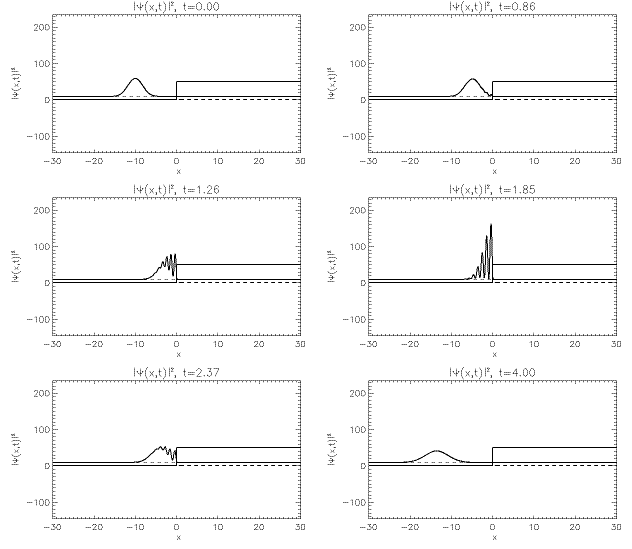
\includegraphics[width=0.5\linewidth]{./lect8/pic1.png}
\end{center}
\subsubsection{Potential well}
\begin{center}
	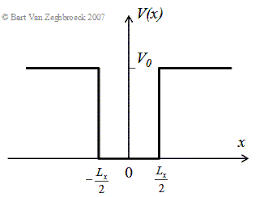
\includegraphics[width=0.4\linewidth]{./lect8/pic2.png}
\end{center}
$$V = \begin{cases}
-V_0 & 0<x<l\\
0 & \text{otherwise}
\end{cases}$$
Thus
$$\psi_E(x) = \begin{cases}
Ae^{\frac{\kappa x}{\hbar}}& x<0\\
Ce^{\frac{ipx}{\hbar}} +De^{\frac{-ipx}{\hbar}} & 0<x<L\\
Be^{\frac{\kappa x}{\hbar}}& x>L\\
\end{cases}$$
From differentiability we can get rid of 2 constants in 0, and from 2 more in $l$. Thus in general, there is no solution, the only case is for specific values of $E$.
\subsubsection{Infinite potential well}
What happens when $V_0 \to \infty$, in this case particle can't leave the well, i.e. $\psi(x)= 0$.
	
So we already have the solution:
$$\psi(x) = \begin{cases}
Ae^{\frac{ipx}{\hbar}} +Be^{\frac{-ipx}{\hbar}} & 0<x<L\\
0 \\ \text{otherwise}
\end{cases}$$
From $\psi(0)=0$ we acquire that
$$\psi(x) = C\sin(\frac{ipx}{\hbar})$$
Since $C\neq=0$ we get that $p$ can aquire only particular values such that
$$\frac{pL}{\hbar} = n\pi$$
$$p=\frac{n\hbar \pi}{2}$$
Thus, since
$$H = \frac{p^2}{2m}$$
$$E_n = \frac{n^2\hbar^2 \pi^2}{2mL^2}$$
and
$$\psi = C \sin(\frac{n \pi x}{L})$$

\subsubsection{General case}
If we have piecewise constant potenetial:

\begin{center}
	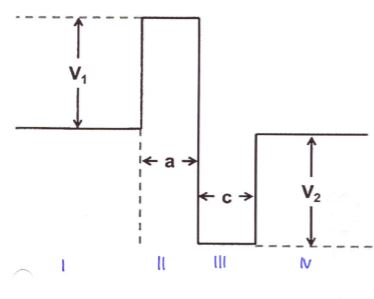
\includegraphics[width=0.4\linewidth]{./lect9/pic1.jpg}
\end{center}
For potential higher than energy we get decaying potential, and for each of wells we get oscillating solution.

\subsection{Bound states}
If we close to potential minimum, we can approximate it with Taylor series as
$$V \approx \frac{1}{2} m\omega^2 X^2$$
We will solve the Schr\"{o}dinger equation for harmonic oscillator:
$$H\ket{\psi_E} = E\ket{\psi_E}$$
For
$$H = \frac{p^2}{2m} + \frac{1}{2} m\omega^2 X^2$$
In position representation we get
$$-\frac{\hbar^2}{2m}\psi_E + \frac{1}{2}mw^2X^2\psi_E = E\psi_E$$
Lets perform variable substitution:
$$a = \sqrt{\frac{m\omega}{2\hbar}} X +i\frac{1}{\sqrt{2m\omega\hbar}} P$$
Since $X$, $P$ are Hermitian
$$a^\dagger = \sqrt{\frac{m\omega}{2\hbar}} X +i\frac{1}{\sqrt{2m\omega\hbar}} P$$
$$a^\dagger a = \frac{mw}{2\hbar}X^2 +\frac{P^2}{2m\omega\hbar } +\frac{1}{2\hbar} i(XP-PX) $$
$$a^\dagger a = \frac{mw}{2\hbar}X^2 +\frac{P^2}{2m\omega\hbar } +\frac{1}{2\hbar} i\comm{X}{P} $$
$$\comm{X}{P} = \hbar\comm{X}{K} = ih$$
Thus
$$H = \hbar \omega \qty(a^\dagger a + \frac{1}{2})$$

Denote $N=a^\dagger a$ and $N\ket{n} = n\ket{n}$. 

We can show that $n\geq 0$ and $$a\ket{n} =\begin{cases}
\ket{n-1}&n\neq0\\
0&n=0
\end{cases}$$
Which means than $n$ has to be integer.
Note that
$$\norm{a\ket{n}} =\mel{n}{a^\dagger a}{n} = \mel{n}{N}{n} = n$$
Thus, if $n=0$, $\norm{a\ket{n}} = 0$, denote this vector as $\ket{0}$ (note that $\norm{\ket{0}}\neq0 $).

Let's show that $a^\dagger \ket{n} \neq 0$. Suppose  exists such $\ket{n}$: 
$$a^\dagger \ket{n} = 0$$
$$aa^\dagger  \ket{n} = 0$$

For that, calculate
$$\comm{a}{ a^\dagger} = \comm{\sqrt{\frac{m\omega}{2\hbar}} X +i\frac{1}{\sqrt{2m\omega\hbar}} P}{ \sqrt{\frac{m\omega}{2\hbar}} X -i\frac{1}{\sqrt{2m\omega\hbar}} P} = \sqrt{\frac{m\omega}{2\hbar}}i\frac{1}{\sqrt{2m\omega\hbar}} \qty( \comm{X}{-P}+\comm{P}{X}) = \frac{i}{2\hbar} (-2i\hbar) = 1$$


Then
$$aa^\dagger = a^\dagger a + 1 = N+1$$

i.e.,
$$(N+1)\ket{n} = (n+1)\ket{n} = 0$$
That means $n=-1$, however $n\geq 0 $.

Lets show that $a^\dagger \ket{n}$ and $a \ket{n} \neq 0 $ are eigenvectors of $N$.

$$Na^\dagger \ket{n} = a^\dagger a a^\dagger \ket{n} = a^\dagger (a^\dagger a+1)\ket{n} = a^\dagger (N+1)\ket{n}= a^\dagger(n+1)\ket{n} = (n+1)a^\dagger \ket{n}$$
We got
$$a^\dagger \ket{n}\propto \ket{n+1}$$

For $a\ket{n}$:
$$Na^\dagger a a \ket{n} = (aa^\dagger -1) a \ket{n} = (aa^\dagger a - a)\ket{a} = a(N-1)\ket{n}= a(n-1)\ket{n} $$
i.e.,
$$a\ket{n} \propto \ket{n-1}$$

We can conclude there doesn't exist $0<n<1$, because then $a\ket{n} \propto \ket{n-1}$ and $N\ket{n-1} = (n-1)\ket{n-1}$ and $n-1<0$ in contradiction.

By induction or just by looking on $a^m\ket{n}$ we can show same for any non-integer $n$.

However for integer $n$, we get 0 at some point, and thus there is no contradiction. And for each $m$, $\qty(a^\dagger)^m \ket{n} = \ket{n+m}$.

We found the spectrum of $N$ and
$$H = \hbar \omega \qty(N+\frac{1}{2})$$
Thus
$$H\ket{n} = \hbar \omega \qty(n+\frac{1}{2})\ket{n}$$
And states $\ket{n}$ are eigenvalues of $H$ with eigenvalues $\hbar \omega \qty(n+\frac{1}{2})$ i.e., energy are discrete.

We want to find
$$\psi_n(x) = \braket{x}{n}$$
First of all we want to find $\psi_0(x) = \braket{x}{0}$. ($\ket{0}$ is called ground state, $\ket{1}$ is called first excited state, etc.)

Since $a\ket{0}=0$,
$$\mel{x}{a}{0} = 0$$
$$\mel{x}{\sqrt{\frac{m\omega}{2\hbar}} X +i\frac{1}{\sqrt{2m\omega\hbar}} P}{0} = 0$$
$$\sqrt{\frac{m\omega}{2\hbar}}x\psi_0(x) +i\frac{1}{\sqrt{2m\omega\hbar}} \qty(-i\hbar \pdv{x}) \psi_0(x)= 0$$
$$\qty(\sqrt{\frac{m\omega}{\hbar}} x + \frac{1}{\sqrt{\frac{m\omega}{2\hbar}} X +i\frac{1}{\sqrt{2m\omega\hbar}} P}\pdv{x})bb\psi_0(x) = 0$$
Define $y=\sqrt{\frac{m\omega}{\hbar}}x$ and $\tilde{\psi}_0(y) = \psi_0(x)$:
$$\qty(y+\pdv{y}) \tilde{\psi}_0(y) = 0$$
$$\pdv{\tilde{\psi}_0}{y} = -y$$
$$\ln \tilde{\psi}_0 = -\frac{1}{2} y^2 + C$$
$$\tilde{\psi}_0 = C e^{-\frac{1}{2} y^2 }$$
$$\psi_0(x)  = C e^{-\frac{m\omega x^2}{2\hbar}}$$
From normalization requirement, $C = \qty(\frac{m\omega}{\pi \hbar})^{\frac{1}{4}}$ (Gaussian integral).

To find $\psi_n(x) = \braket{x}{n}$ we use the fact $(a^\dagger)^n \ket{0} \propto \ket{n}$.
For that we need the constant  factor:
$$1 = \braket{n+1}{n+1} = \frac{\mel{n}{aa^\dagger}{n}}{\abs{C_n}^2} = \frac{\mel{n}{N+1}{n}}{\abs{C_n}^2} = \frac{n+1}{\abs{C_n}^2}  $$

Since we have freedom of choice of phase, we can choose $C_n = \sqrt{n+1}$.

Thus
$$\psi_n(x) = \mel{x}{\frac{\qty(a^\dagger)^n}{\sqrt{n!}}}{0}$$
Substituting
$$\psi_n(x) =\frac{1}{\sqrt{n!}}\qty(\sqrt{\frac{m\omega}{2\hbar}} X +i\frac{1}{\sqrt{2m\omega\hbar}} P)^n \psi_0(x)$$
$$\tilde{\psi}_n(y) = \frac{1}{\sqrt{n!}} \qty(\frac{1}{\sqrt{2}}\qty(y-\pdv{y}))^n \tilde{\psi}_0(y)$$

Define $\tilde{H}_n$ such that
$$\tilde{\psi}_n(y) = \frac{1}{\sqrt{2^nn!}} \tilde{\psi_0}(y) \tilde{H}_n(y)$$
i.e.,
$$\tilde{H}_n(y) = \frac{1}{\tilde{\psi}_0(y)} \qty(y-\pdv{y})^n\tilde{\psi}_0(y)$$
$$\tilde{H}_n(y) = e^{\frac{1}{2}y^2} \qty(y-\pdv{y})^n  e^{-\frac{1}{2}y^2} $$

\paragraph{Values of $\tilde{H}_n$}
$$\tilde{H}_0(y) = 1$$
$$\tilde{H}_1(y) = e^{\frac{1}{2}y^2} \qty(y-\pdv{y})  e^{-\frac{1}{2}y^2} = y + y e^{\frac{1}{2}y^2}e^{-\frac{1}{2}y^2} = 2y $$

i.e., we found general expression:
$$\psi_n(x) = \frac{1}{\sqrt{2^nn!}} \tilde{H}_n\qty(\sqrt{\frac{m\omega}{\hbar}}x)\qty(\frac{m\omega}{\pi \hbar})^{\frac{1}{4}}e^{-\frac{m\omega x^2}{2\hbar}}$$

For initial state we rewrite
$$\psi(x,0) = \sum_n c_n \psi_n(x)$$
and from normalization
$$\int_{-\infty}^{\infty} \dd{x} \psi^*_{n'} (x) \psi_n(x)  = \braket{n}{n'} = \delta_{nn'}$$
we get
$$c_n = \int_{-\infty}^\infty \dd{x} \psi^*(x) \psi(x,0)  $$
And we get
$$\psi(x,t) = \sum_n c_n e^{-\frac{i(\hbar \omega \qty(n+\frac{1}{2}))t}{\hbar}} \psi_n(x)$$
\section{General properties in one dimension}
\paragraph{In one dimension, bound states are non degenerated}
$$H = \frac{P^2}{2m} + V(x)$$
Suppose $\psi_1$ and $\psi_2$ are two eigenvectors of eigenvalue $E$. Let's show that $\psi_1$ and $\psi_2$ are same eigenvector up to normalization. We know that
$$\qty(\frac{P^2}{2m} + V(x)) \ket{\psi_i} = E \ket{\psi_i}$$
Choose $i=1$, and multiply by $\psi_2$
$$\psi_2\qty(-\frac{\hbar}{2m}\pdv[2]{x}\psi_1) + V\psi_2\psi_1 = E\psi_2\psi_1$$
and similarly
$$\psi_1\qty(-\frac{\hbar}{2m}\pdv[2]{x}\psi_2) + V\psi_2\psi_1 = E\psi_2\psi_1$$
Subtracting 
$$\psi_2 \pdv[2]{x} \psi_1 - \psi_1 \pdv[2]{x} \psi_2 = 0$$
$$\qty(\psi_2 \pdv[2]{x} \psi_1 + \pdv{x}\psi_1\pdv{x}\psi_2) - \qty(\psi_1 \pdv[2]{x} \psi_2 + \pdv{x}\psi_1\pdv{x}\psi_2)= 0$$
$$\pdv{x} \qty(\psi_2\pdv{x}\psi_1 - \psi_1\pdv{x}\psi_2) = 0$$
And thus
$$\psi_2\pdv{x}\psi_1 - \psi_1\pdv{x}\psi_2 = C$$
Since states are bounded, $\psi_i \stackrel{x\to \pm \infty}{\longrightarrow} 0$, for $x\to \pm \infty$, $\psi_2\pdv{x}\psi_1 - \psi_1\pdv{x}\psi_2 =0$, and thus $C=0$.
$$\psi_2\pdv{x}\psi_1 - \psi_1\pdv{x}\psi_2 = 0$$
$$\psi_2\pdv{x}\psi_1 = \psi_1\pdv{x}\psi_2 $$
$$\ln \psi_1 = \ln \psi_2 + \tilde{C} $$
$$\psi_1 =  e^{\tilde{C}} \psi_2 $$
i.e., there is no degeneracy. This is right only for one dimension and specific Hamiltonian.
\subsection{Ehrenfest theorem and classical limit}
$$\begin{cases}
\dv{t} \expval{X} = \expval{\pdv{H}{P}}\\
\dv{t} \expval{P} = -\expval{\pdv{H}{X}}\\
\end{cases}$$
\paragraph{Ehrenfest theorem}
For time-independent $\Omega$ 
$$\dv{t} \mel{\phi}{\Omega}{\psi} = -\frac{i}{\hbar} \mel{\phi}{\comm{\Omega}{H}}{\psi}$$
\subparagraph{Proof}
$$\dv{t} \mel{\phi}{\Omega}{\psi}  = \qty(\dv{t} \bra{\phi}) \Omega \ket{\psi} + \mel{\phi}{\dv{t}\Omega}{\psi} +  \bra{\phi} \Omega \qty(\dv{t}\ket{\psi})$$
From Shr\"{o}dinger equation

$$\dv{t} \mel{\phi}{\Omega}{\psi}  = \frac{i}{\hbar} \bra{\phi} H \Omega \ket{\psi} + \mel{\phi}{\dv{t}\Omega}{\psi} +  \frac{i}{\hbar}\bra{\phi} \Omega H\ket{\psi} =-\frac{i}{\hbar} \mel{\phi}{\comm{\Omega}{H}}{\psi} + \mel{\phi}{\dv{t}\Omega}{\psi} $$
\paragraph{}
For Hamiltonian of form
$$H = \frac{P^2}{2m} + V(x)$$
$$\dv{t}\expval{X} = -\frac{i}{\hbar} \expval{\comm{X}{H}}$$
Since each function of operator commutes with operator
$$\dv{t}\expval{X} = -\frac{i}{\hbar} \expval{\comm{X}{\frac{P^2}{2m}}}$$
$$\comm{X}{P^2} =P\comm{X}{P} + \comm{X}{P}P = 2i\hbar P$$
$$\dv{t} \expval{X} = -\frac{i}{\hbar} \frac{1}{2m} 2i\hbar \expval{P} $$
$$\dv{t} \expval{X} =  \frac{\expval{P}}{m}   $$

For more general case
$$H(X,P) = \sum_{n,m} a_{nm} X^nP^m$$
We want to calculate $\comm{X}{H}$
$$\comm{X}{H} = \comm{X}{\sum_{n,m} a_{nm} X^nP^m} = \sum_{n,m} a_{nm}\comm{X}{ X^nP^m} = \sum_{n,m} a_{nm}\qty(X^n\comm{X}{ P^m}+\comm{X}{X^n }P^m)  = \sum_{n,m} a_{nm}X^n\comm{X}{ P^m}$$
We can show by induction that $\comm{X}{ P^m} = mi\hbar P^{m-1}$ and then
$$\comm{X}{H} =  i\hbar  \expval{\pdv{H}{P}}$$
and

$$\dv{t} \expval{X} =  \expval{\pdv{H}{P}} $$

For $P$ we get $\dv{t} \expval{P} = -i\hbar \expval{\comm{P}{H}}$.
$$\comm{P}{H} = \comm{P}{\sum_{n,m} a_{nm} X^nP^m} = \sum_{n,m} a_{nm}\comm{P}{ X^n}P^m$$
$$\comm{P}{X} = -i\hbar$$
By induction we can show $\comm{P}{X^n} = -ni\hbar X^{n-1}$.
$$\comm{P}{H} = \sum_{n,m} -a_{nm}ni\hbar X^{n-1}P^m = -i\hbar \pdv{H}{X}$$
\paragraph{} Take a look at $H = \frac{P^2}{2m} + V(X)$ such that $\pdv{H}{X} = V'(X)$. Define $x_0 = \expval{X}$ such that
$$V'(X) = V'(x_0) I + (X-Ix_0)V''(x_0) + \frac{1}{2}(X-Ix_0)^2V'''(x_0) + \dots$$
We want to compare $V'(\expval{X})$ and $\expval{V'(X)}$.
$$\expval{V'(X)} = V'(x_0) + (x_0-x_0)V''(x_0) + \frac{1}{2} \Delta x^2 V'''(x_0)+\dots = V'(x_0) +\frac{1}{2} \Delta x^2 V'''(x_0)+\dots$$

We've got that classical equations can be applied if $\Delta x^2$ is small.
\end{document}
